\documentclass{article}
\usepackage[utf8]{inputenc}
\usepackage[english,russian]{babel}
\usepackage{amssymb,amsthm,amsmath,amscd}
\usepackage{graphicx}
\graphicspath{ {images/} }
\usepackage{float}
\usepackage{subcaption}
\usepackage{hyperref}

\title{
    ОЭДвСС\\
    Цифровая обработка сигналов\\
    Лабораторная работа 1
}
\author{Ivan Pazhitnykh}
\date{November 2018}

\begin{document}
\maketitle

\section{Определить период сигнала:}
\begin{equation}
    x(t) = 2\sin(2\pi 3t)+3\sin(2\pi 5t)+6\sin(2\pi 8t)
\end{equation}

Находим НОД частот:
\begin{equation*}
    f = gcd(3, 5, 6) = 1\:(Hz.)
\end{equation*}

Вычисляем период:
\begin{equation*}
    T = \frac{1}{f} = 1\:(s.)
\end{equation*}

\section{Определить min частоту дискретизации:}

\textbf{max} частотная составляющая дискретизации непрерывного сигнала равна 5000 (Гц)

\begin{equation*}f_{max} = 5000\end{equation*}
\begin{equation*}f_{min} - ?\end{equation*}

В соответствии с теоремой \textbf{\href{http://bit.ly/2AknLuQ}{Котельникова}} (связывает непрерывные и дискретные сигналы):

\begin{equation*}
    f_{min} = 2f_{max} = 2 * 5000 = 10000\:(Hz.)
\end{equation*}

\newpage
\section{Построить амплитудный спектр графика:}
\begin{figure}[h]
    \centering
    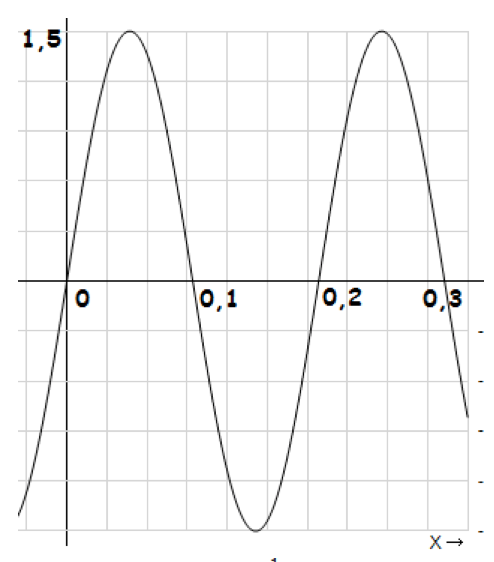
\includegraphics[width=0.5\textwidth]{task3.png}
\end{figure}

Амплитуда $A = 1.5$, найдём частоту:
\begin{equation*}
    f = \frac{1}{T} = \frac{1}{0.2} = 5\:(Hz.)
\end{equation*}
\begin{figure}[h]
    \centering
    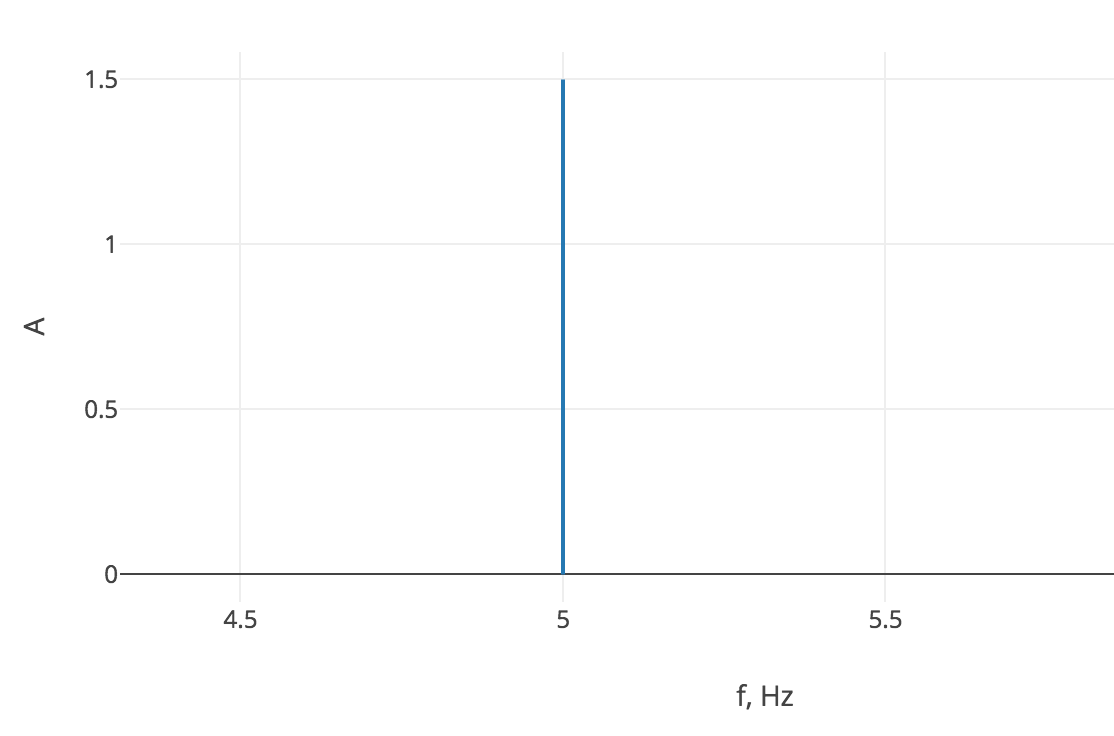
\includegraphics[width=0.8\textwidth]{plot3.png}
    \caption{Амплитудный спектр}
\end{figure}

\newpage
\section{Построить амплитудный спектр графика:}
\begin{figure}[h]
    \centering
    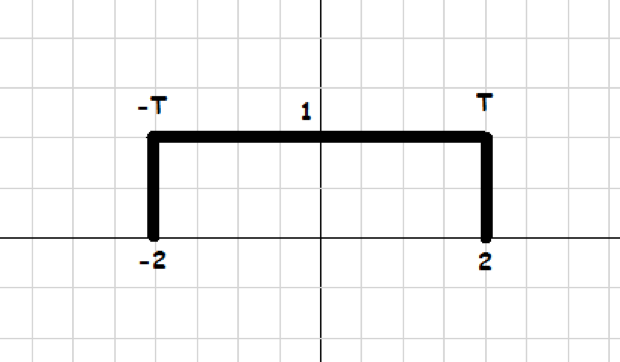
\includegraphics[width=0.7\textwidth]{task4.png}
\end{figure}

\begin{equation}
    x(t) = 1,\:-T < t < T;\:0,\:otherwise
\end{equation}

Найдём спектр прямоугольного импульса через прямое преобразование Фурье:
\begin{equation*}
    X(f) = 2T\frac{\sin(2\pi f T)}{2\pi f T} = \frac{\sin(2\pi f T)}{\pi f}
\end{equation*}

\begin{equation*}
    \lim_{f\to{x}}X(f) = 2T
\end{equation*}

Функция обращается в ноль в: 
$\pm\frac{1}{2T}, \pm\frac{2}{2T}, \pm\frac{3}{2T},...$,
$X(0) = 2T = 4$

\begin{figure}[h]
    \centering
    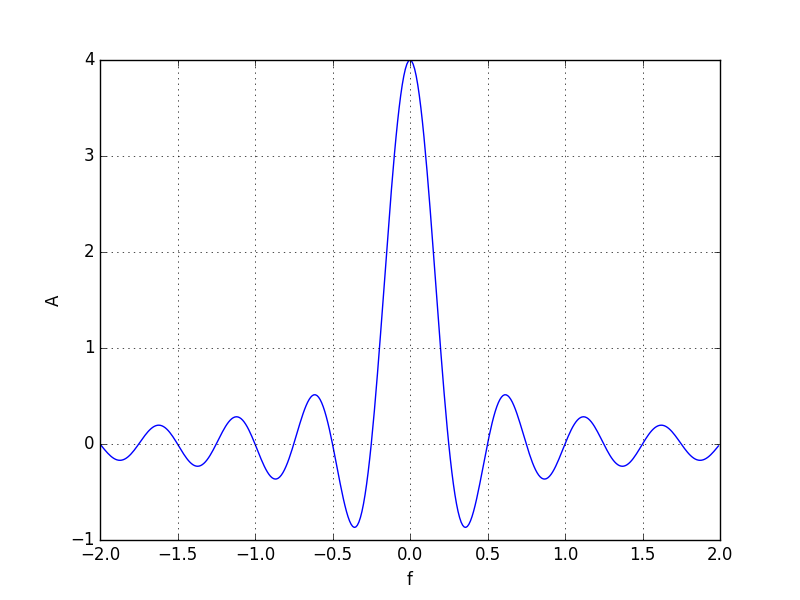
\includegraphics[width=0.75\textwidth]{plot4.png}
    \caption{Амплитудный спектр}
\end{figure}

\newpage
\section{Записать выражение сигнала:}
\begin{figure}[h]
    \centering
    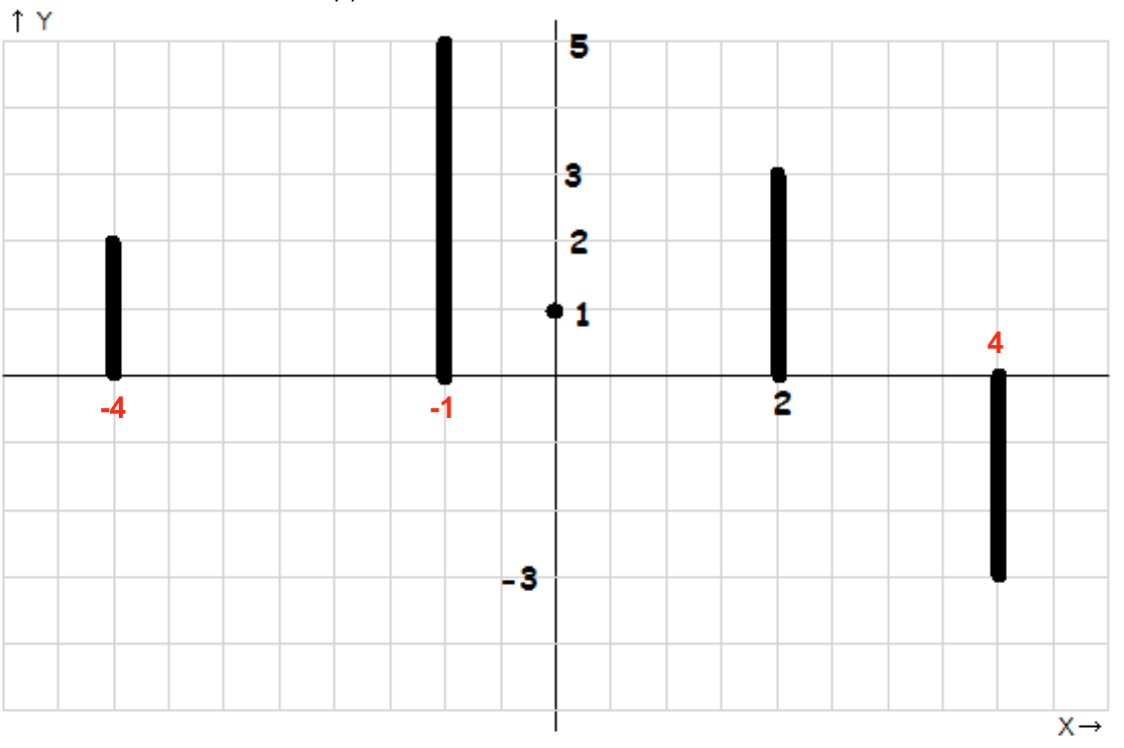
\includegraphics[width=0.8\textwidth]{task5.png}
\end{figure}

Запишем дельта-функцию:
\begin{equation*}
    \delta(t-n) = 0,\:if\:t\ne n
\end{equation*}

Таким образом: $t-n=4 \rightarrow t=n+4$, следовательно:

\begin{equation*}
    x(n) = 2\delta(n+4) + 5\delta(n+1) + \delta(n) + 3\delta(n-2) - 3\delta(n-4)
\end{equation*}

\section{Построить сигнал по выражению:}
\begin{equation}
    x(n) = 3\delta(n+3) - 6\delta(n+1) + \delta(n) + 3\delta(n-3) - 3\delta(n-5)
\end{equation}
\begin{figure}[h]
    \centering
    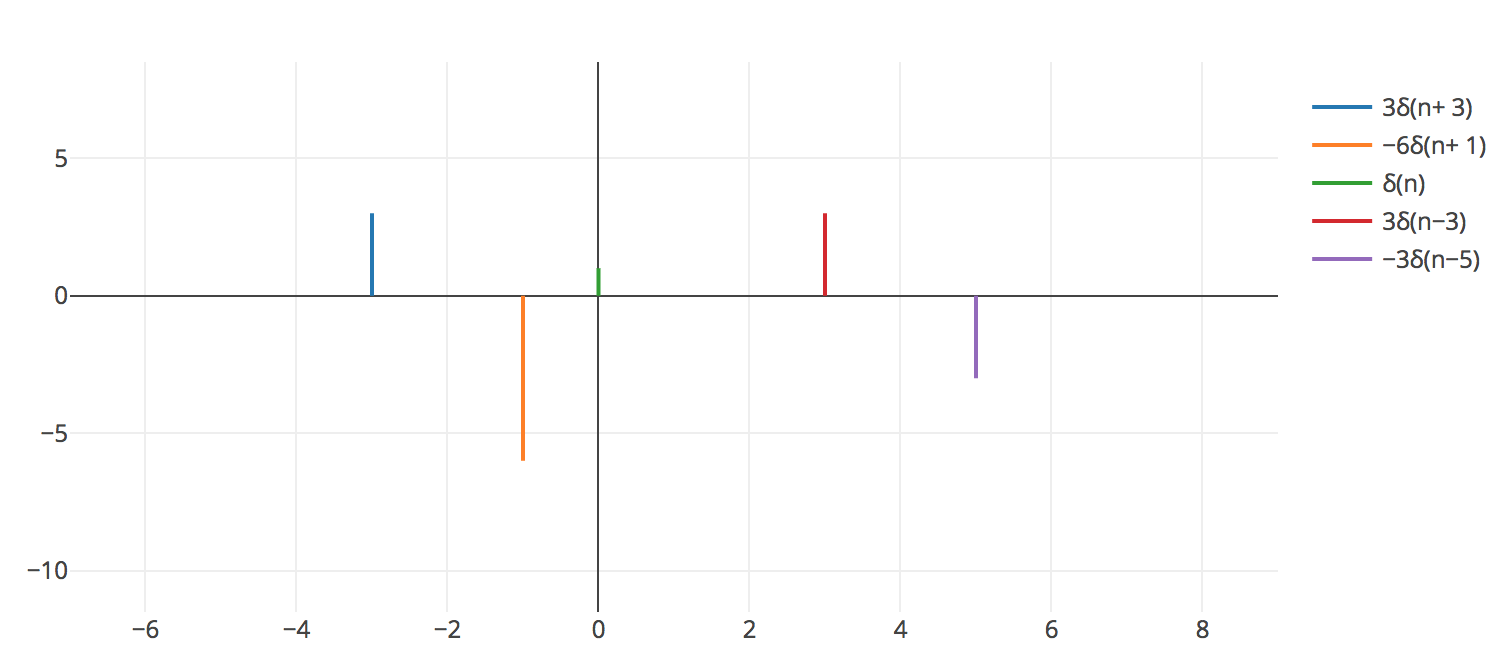
\includegraphics[width=1\textwidth]{plot6.png}
\end{figure}

\newpage
\section{Задача:}
Для измерения давления используется датчик с коэффициентом преобразования \textbf{50 мВ/Па}.
На выходе датчика напряжение \textbf{10500 мВ}. Определить измеряемое давление.

$P_{\text{вых}} -?$

$K_{\text{пр}} = 50\:(\frac{\text{мВ}}{\text{Па}})$

$U_{\text{вых}} = 10500 \text{ (мВ)}$

$P_{\text{вых}} = \frac{U_{\text{вых}}}{K_{\text{пр}}} = 210 \text{ (Па)}$

\section{Построить амплитудный спектр сигнала:}
\begin{equation}
    x(t) = 5\sin(2\pi 2t) + 6\cos(2\pi 8t) +4\sin(2\pi 10t)
\end{equation}

\begin{figure}[h]
    \centering
    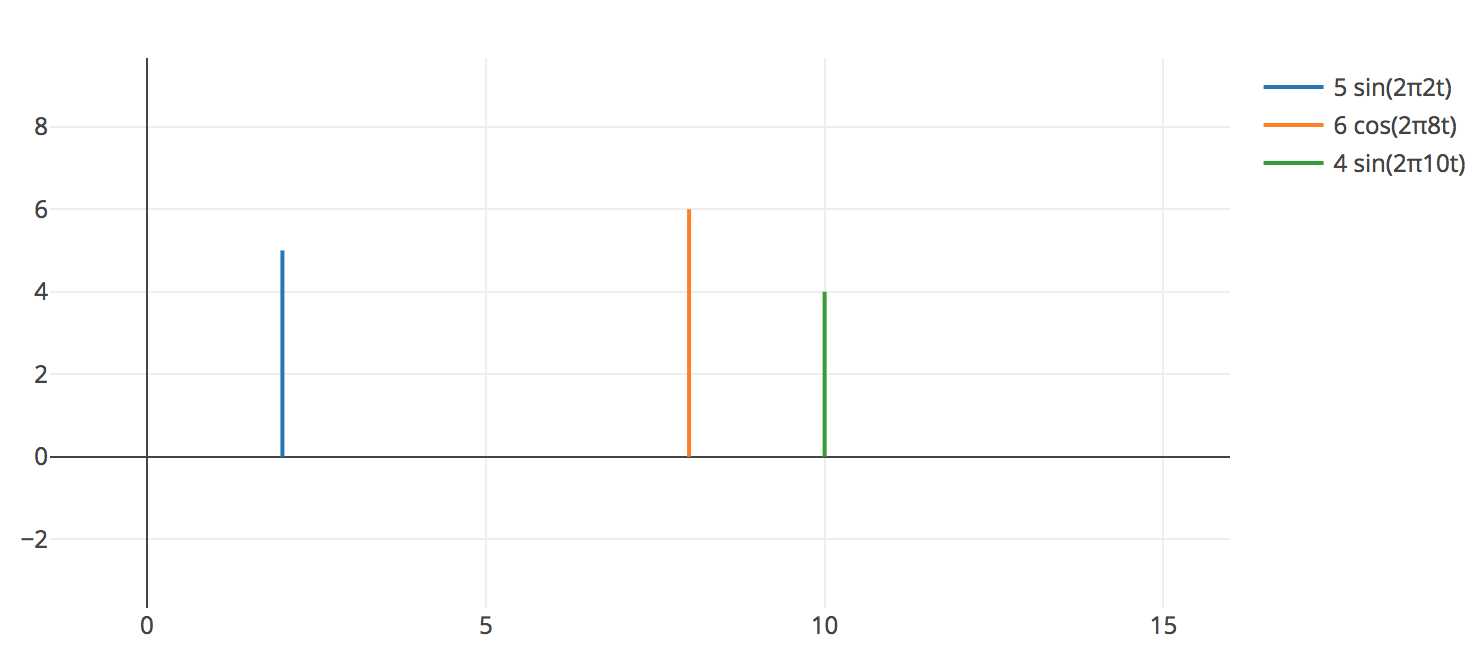
\includegraphics[width=1\textwidth]{plot8.png}
\end{figure}

\end{document}
